\documentclass[a4paper, 12pt]{article}

\usepackage{amsmath}
\usepackage{amssymb}
\usepackage{vector}
\usepackage{cite}
\usepackage{graphicx}
\usepackage{subfig}
\usepackage[usenames, dvipsnames]{color}

\usepackage{setspace}
\usepackage{fancyhdr}
\usepackage{ifthen}
\usepackage{ifpdf}
\usepackage{float} 

\usepackage[english]{babel}

%-->
%--> Google.com search "hyperref options"
%--> 
%--> http://www.ai.mit.edu/lab/sysadmin/latex/documentation/latex/hyperref/manual.pdf
%--> http://www.chemie.unibas.ch/~vogtp/LaTeX2PDFLaTeX.pdf 
%--> http://www.uni-giessen.de/partosch/eurotex99/ oberdiek/print/sli4a4col.pdf
%--> http://me.in-berlin.de/~miwie/tex-refs/html/latex-packages.html
%-->
\usepackage[ pdftex, plainpages = false, pdfpagelabels, 
             pdfpagelayout = useoutlines,
             bookmarks,
             bookmarksopen = true,
             bookmarksnumbered = true,
             breaklinks = true,
             linktocpage,
             pagebackref,
             colorlinks = false,
             linkcolor = blue,
             urlcolor  = blue,
             citecolor = red,
             anchorcolor = green,
             hyperindex = true,
             hyperfigures
             ]{hyperref} 
\usepackage{graphicx}
%\pdfcompresslevel=9
\DeclareGraphicsExtensions{.png, .jpg, .pdf}


\pdfpageheight=297mm
\pdfpagewidth=210mm

\setlength{\hoffset}{0.00cm}
\setlength{\voffset}{0.00cm}

%\setlength{\evensidemargin}{1.96cm}
%\setlength{\oddsidemargin}{-0.54cm}
%% \setlength{\topmargin}{1mm}
%% \setlength{\headheight}{1.36cm}
%% \setlength{\headsep}{1.00cm}
%% \setlength{\textheight}{20.84cm}
%% \setlength{\textwidth}{14.5cm}
%% \setlength{\marginparsep}{1mm}
%% \setlength{\marginparwidth}{3cm}
%% \setlength{\footskip}{2.36cm}


% \pagestyle{fancy}
% \renewcommand{\sectionmark}[1]{\markright{#1}{}}
% \fancyhf{}
% \fancyhead[RO]{\bfseries\rightmark}
% \fancyhead[LE]{\bfseries\leftmark}
% \fancyfoot[C]{\thepage}
% \renewcommand{\headrulewidth}{0.5pt}
% \renewcommand{\footrulewidth}{0pt}
% \addtolength{\headheight}{0.5pt}
% \fancypagestyle{plain}{
%   \fancyhead{}
%   \renewcommand{\headrulewidth}{0pt}
% }



% The year and term the degree will be officially conferred
\def\degreedate#1{\gdef\@degreedate{#1}}
% The full (unabbreviated) name of the degree
\def\degree#1{\gdef\@degree{#1}}
% The name of your college or department(eg. Trinity, Pembroke, Maths, Physics)
\def\collegeordept#1{\gdef\@collegeordept{#1}}
% The name of your University
\def\university#1{\gdef\@university{#1}}
% Defining the crest
\def\crest#1{\gdef\@crest{#1}}


%define title page layout
\renewcommand{\maketitle}{%
    \renewcommand{\footnotesize}{\small}
    \renewcommand{\footnoterule}{\relax}
    \thispagestyle{empty}
%  \null\vfill
  \begin{center}
    { \Huge {\bfseries {Numerical Methods \\for Deforming Images}} \par}
{\large \vspace*{25mm} {\includegraphics[width=35mm]{img/imperial_crest} \par} \vspace*{22mm}}
    {{\Large \bfseries{\href{mailto:rjcrim@gmail.com}{Robert Crim}}} \par}
{\large \vspace*{1ex}
    {\href{http://www.ic.ac.uk/aeronautics}{Department of Aeronautics} \par}
\vspace*{1ex}
    {\href{http://www.ic.ac.uk}{Imperial College London} \par}
\vspace*{20mm}
    {\small Submitted in part fulfillment of the requirements for the degree of} \par}
\vspace*{0.5ex}
    {\large \it{Master of Science} \par}
\vspace*{1ex}
    {16 September 2011}
  \end{center}
  \null\vfill
}


\newcommand{\eq}[1]{(\ref{eq:#1})}
\newcommand{\fig}[1]{Fig. \ref{fig:#1}}
\newcommand{\vect}[1]{\ensuremath{\mathbf{#1}}}
\newcommand{\hvect}[1]{\ensuremath{\hat{\vect{#1}}}}

\newcommand{\pp}[2]{\frac{\partial #1}{\partial #2}}
\newcommand{\vv}[2]{\frac{\delta #1}{\delta #2}}
\newcommand{\angles}[1]{\left\langle #1 \right\rangle}
\newcommand{\eps}{\varepsilon}
\setlength{\parskip}{.3cm}


%\usepackage{mathpazo}
%\usepackage[mathpazo]{flexisym}

%\usepackage{breqn}

%\graphicspath{{./img/}}

% \pdfpagewidth=\paperwidth 
% \pdfpageheight=\paperheight



\begin{document}

\maketitle
\newpage

\pagestyle{plain}
\setcounter{page}{1}
\pagenumbering{roman}

\begin{abstract}
  An image of a continuous closed curve immersed in $\mathbb{R}^2$ is
  transformed from a template curve to a target curve directly. The project
  presents a framework to solve problems with applications in image processing
  and computational anatomy. A time dependent velocity field directly on a
  closed curve, a functional analogous to kinetic energy can be defined using an
  inner metric matching approach. The velocity deforms the template into the
  target over a fixed time interval and the resulting functional can minimised
  using an optimisation algorithm, giving the shortest path, or geodesic,
  between the two shapes.

The formulation of the
  functional and its gradient is shown, along with how the problem is
  discretised for use with a finite element method. Python is used to write a code
  to implement the scheme, which uses the FEniCS and SciPy libraries. The
  results of the code show the approach is valid and shows promise for
  future work. Large deformations are found successfully, despite the scheme not
  being completely parametric invariant.

\end{abstract}
\newpage
\tableofcontents
\newpage

\pagestyle{plain}
\setcounter{page}{1}
\pagenumbering{arabic}

\onehalfspacing
\section{Introduction}

Computational anatomy is a discipline which aims to analyse biological shapes to
determine variability across populations, ages, species, and in the presence of
disease \cite{miller2001group, miller2009emerging}. It is hoped that the ability
to correlate this variability with other anatomical information will aid in the
early diagnosis of disease \cite{mfca11}.

The study of how one image is deformed into another image is of fundamental
importance to computational anatomy. Given two shapes known as the ``template'' and
``target'', the goal is find a relative deformation which makes the template
take the same form as the target. Since there are infinitely many paths to
deform one shape to another --- the shortest path, or geodesic, between the
template and target is desired. The deformation is characterised as a
time-dependent velocity, defining a flow which changes one shape to another over
a fixed time interval. This allows us to express the deformation in terms of
kinetic energy, and the problem becomes one of finding a velocity field that
minimises this energy functional, while ensuring the template deforms into the
target shape \cite{beg2005computing}. 

A method commonly used in comparison of anatomical shapes is the large deformation
diffeomorphic metric matching (LDDMM) based on \cite{grenander1993general}
and developed further in
\cite{beg2005computing,bruveris2011momentum,glaunes2008large}. This approach
involves finding a diffeomorphism which transforms the entire space to match the
template to the target. 

The current report uses an approach based on \emph{inner metrics}, first applied in
in \cite{bauer2011new} which developed from
\cite{michor2005vanishing,michor2003riemannian,younes2008metric}, where the
deforming vector is defined directly on the image itself (\fig{inner_metric}), as opposed to the
\emph{outer metrics} used in LDDMM in which deforming vector is applied to the
entire field (\fig{outer_metric}). An inner metric is defined to determine a path between the
template and target shapes, which when minimised, results in the geodesic
(discretisation dependent) between the two shapes.

\begin{figure}[h!]
  \centering
  \subfloat[Inner metrics \label{fig:inner_metric}]{
    \includegraphics[width=.5\textwidth]{../misc/inner_field.pdf}}
  \subfloat[Outer  metrics \label{fig:outer_metric}]{
    \includegraphics[width=.5\textwidth]{../misc/outer_field.pdf}}
  \caption{Velocity field as defined and with inner metrics (a), where the
    deformation occurs directly on the shape itself, and with outer metrics
    (b), where the vector deforms the entire space.}
  \label{fig:metrics}
\end{figure}

Both the inner metric and outer metric registration methods above are applied to
matching shapes embedded in $\mathbb{R}^3$. We are interested in matching closed
curves immersed in $\mathbb{R}^2$, although the technique can be applied to
surfaces.


We establish a functional $S[\vect{u}]$ for a velocity field $\vect{u}$ by
combining an appropriate metric for $\vect u$ with matching (penalty)
functional. We then use variational calculus and an adjoint equation to derive an
expression for the gradient of $S[\vect{u}]$. This gives us a constrained
nonlinear optimisation problem, for which a BFGS algorithm from the Python
SciPy\cite{scipy} library is used. This takes the functional and its gradient
and attempts to find a velocity $\vect u$ that minimises $S[\vect u]$.


In the registration and subsequent matching of curves, the parameterisation of
the template and target are important. The only interest is in matching the
shape of the template to the target, regardless of how the curves are
parameterised. In other words, if the template is a circle and the target is a
similar circle with the same radius and centre, but rotated by $45^{\circ}$,
then the two shapes are considered identical by a parameterisation invariant
metric. 

Parameterisation invariant 2D matching based on outer metrics was developed in
\cite{cotter2009geodesic, cotter2009curves, clark2011reparam}, and solve an
equation for the geodesic on outer metric space, by finding the initial
conditions using a shooting method.

The approach presented here differs in that it is based on inner metrics, the
penalty term is \emph{not} parameterisation invariant, and that the
functional and its gradient are computed directly by finding the
progression of the shape at each time step.


We attempt to determine the overall applicability of this solution approach, and
provide a framework for further development of the metric and the introduction
of a parameterisation invariant penalty term. The report is organised by first
discussing the formulation of the metric in Sec. \ref{sec:equations}, followed
by the discretisation of the equations needed for the solver in
Sec. \ref{sec:disc}. Notes on the implementation of the finite element method
using FEniCS are provided in Sec. \ref{sec:implementation}. The results of numerical
experiments using the solver are discussed in
Sec. \ref{sec:experiments}. Finally, an outlook and suggestions for further work
are provided in Sec. \ref{sec:conc}


\section{Mathematical formulation \label{sec:equations}}

For the formulation of the problem and in the numerical scheme, a closed curve
on a plane is represented as continuous periodic functions  $\vect q(s),\, s \in [0,2\pi]$ such that
$\vect q(0) = \vect q(2\pi)$.

Given the closed curves $C_{A}$ and $C_B$, the template and targets are
parameterised respectively as
\begin{equation}
  \label{eq:qAqB}
  \vect q_{A}(s),\; \vect q_{B}(s),\; s \in [0,2\pi]
\end{equation}

A time dependent vector field $\vect u(s,t)$ is applied directly to a function
$\vect q(s,t)$ subject to
\begin{equation}
  \vect q_A(s) =\vect q(s,0)   \label{eq:template}
\end{equation}
and with the dynamical constraint
\begin{equation}
  \frac{\partial \vect q}{\partial t}(s,t) = \vect u(s,t) ,\; t \in [0,1]  \label{eq:dqdt}
\end{equation}

We must form a functional that both provides a metric for $\vect u$ and some
measure of how close the deformed curve $\vect q$ is the target $\vect q_B$,
which will allow us to minimise the velocity while ensuring the template  $\vect
q_A$ is deformed into $\vect q_B$. 

The first part of this
functional is a parameterisation invariant metric based on $H^1$-norm
$||f(x)||^2_{H^1} = \int_{\mathbb{R}^2} |f(x)|^2 + |\nabla f(x)|^2\,dx$,
adapted from the metric used in \cite{bauer2011new} for surfaces
\begin{equation}
  \label{eq:metric}
  E[\vect u] = \frac{1}{2} \int^{1}_{t=0} \int^{2\pi}_{s=0}\left( \left| \vect u(s,t) \right|^2 
  \left| \frac{\partial \vect q}{\partial s} \right|  + 
  \alpha^2 \frac{ 
    \left| \frac{\partial \vect u}{\partial s}\right|^2}{
    \left| \frac{\partial \vect q}{\partial s}\right|}\right)  \,ds\,dt.
\end{equation}
This provides us with a generalised $H^1$-type norm for $\vect u$, which only
depends on the image itself, regardless of its parameterisation
\cite{bauer2011new}.  Where the constant $\alpha$ in \eq{metric} is a problem
specific a parameter which controls the characteristic length scale of the
deformations.

We introduce a penalty term, or matching functional, to enforce to the ``soft''
constraint that $\vect q(s,1) \rightarrow \vect q_B(s)$ through time.
\begin{equation}
  \label{eq:penalty}
  d(\vect q(s,1),\vect q_B) = \frac{1}{2\sigma^2}\int^{2\pi}_{s=0}\left| \vect q(s,1) -
    \vect q_B(s)\right|^2\,ds
\end{equation}
This is based on the squared $L^2$ distance between the shapes, with the
addition of the $\sigma$ constant. The parameter $\sigma$ allows the
``importance'' of the penalty term relative to the metric to be controlled,
since there will likely be an acceptable error between $\vect q_B$ and $\vect q(s,1)$.

We can combine the metric \eq{metric} and penalty \eq{penalty} terms to
state the optimisation problem for the functional $S[\vect u]$ as
\begin{equation}
  \begin{split}
  \label{eq:S}
  \min_{\vect u} S[\vect u] = \frac{1}{2} \int^{1}_{0} \int^{2\pi}_{0}\left| \vect u(s,t) \right|^2 
  \left| \frac{\partial \vect q}{\partial s} \right|  + 
  \alpha^2 \frac{ 
    \left| \frac{\partial \vect u}{\partial s}\right|^2}{
    \left| \frac{\partial \vect q}{\partial s}\right|} \,ds\,dt \\
  + \frac{1}{2\sigma^2}\int^{2\pi}_{0}\left| \vect q(s,1) - \vect q_B(s)\right|^2\,ds.
  \end{split}
\end{equation}

Strictly speaking, the functional $S$ is all that is needed for the problem and
could potentially be used alone with an optimisation algorithm. However, finding the
velocity that minimises $S$ is significantly faster with its gradient known. We can find this from the variational derivative
\begin{equation}
  \label{eq:lim_dS}
  \int^1_0 \vv{S}{\vect u}\cdot \delta \vect u\,dt = 
  \lim_{\eps \rightarrow 0} \frac{S[\vect u + \eps \delta \vect u] - S[\vect u]}{\eps},
\end{equation}
 however it is difficult to find $\vv{S}{\vect u}$ directly. Since we can find $\vv{S}{\vect q}$, a Lagrange multiplier can be used find $\vv{S}{\vect u}$.

Relaxing the constraint \eq{dqdt} and introducing the Lagrange multiplier $\hvect q$, $S[\vect u]$ can be reformulated as
\begin{equation}
  \label{eq:J}
  J[\vect q, \vect u, \hvect q] = S[\vect u] + \int^1_0\left\langle \hvect q ,\pp{q}{t} - \vect u\right\rangle \,dt
\end{equation}
with the bra-ket notion for inner product over the interval $(0,2\pi)$ with respect to $s$,
\begin{equation}
  \left\langle f(s),g(s) \right\rangle := \int^{2\pi}_0 f(s) \cdot g(s)\,ds.
\end{equation}
If $\vect u$ is chosen to satisfy \eq{dqdt}, then
\begin{equation}
  \label{eq:JeqS}
  J[\vect u, \vect q, \hvect q] \equiv S[\vect u].
\end{equation}
By setting $\pp{J}{\hvect q} = 0$, \eq{dqdt} is satisfied and the derivative of \eq{JeqS} is
\begin{equation}
  \label{eq:dSeqdJ}
  \pp{S}{\vect u} =  \pp{J}{\vect u} + \pp{J}{\vect q}\cdot\pp{\vect q}{\vect u}
\end{equation}

We first find an equation for  $\vv{J}{q}$ using the definition of the functional derivative \eq{lim_dS}
\begin{equation}
  \label{eq:lim_dJdq}
  \left\langle \vv{J}{\vect q}, \delta \vect q \right\rangle =
  \lim_{\eps \rightarrow 0} \frac{J[\vect u, \vect q + \eps \delta \vect q, \hvect q] - J[\vect u, \vect q, \hvect q]}{\eps}
\end{equation}
Expanding the right side of \eq{lim_dJdq} and taking only $O(\eps)$ terms gives
\begin{equation}
  \begin{split}
  \label{eq:dJdq}
  \left\langle \vv{J}{\vect q}, \delta \vect q \right\rangle =
  \frac{1}{2}\int^1_0\int^{2\pi}_0 |\vect u|^2
  \frac{\pp{}{s}\delta \vect q \cdot \pp{\vect q}{s}}{|\pp{\vect q}{s}|}
    + \alpha^2 \frac{|\pp{\vect u}{s}|^2}{|\pp{\vect q}{s}|^3} \pp{}{s}\delta \vect q \cdot \pp{\vect q}{s} \,ds\,dt  \\
    + \left\langle \delta \vect q, \vect q\big|_{t=1} - \vect q^B \right\rangle + \int^1_0\left\langle \hvect q, \pp{}{t} \delta \vect q \right\rangle\,dt
\end{split}
\end{equation}
Using the property of adjoint equations $\pp{}{t}\angles{x,y} = \angles{\dot x, y} + \angles{x, \dot y}$, we can write

\begin{equation}
\begin{split}
  \label{eq:adjoint}
  \int^1_0\angles{\hvect q, \delta \pp{}{s} \vect q}\,dt &=  
  \int^1_0\angles{\frac{d}{dt}\hvect q, \delta \vect q}\,dt -  \int^1_0\angles{\pp{\hvect q}{t}, \delta \vect q }\,dt  \\
  &= \int^1_0\angles{\frac{d}{dt}\hvect q, \delta \vect q}\,dt - \Big[\angles{\hvect q, \delta \vect q}\Big]^1_0  \\
  &= \int^1_0\angles{\frac{d}{dt}\hvect q, \delta \vect q}\,dt - \angles{\hvect q\big|_{t=1}, \delta \vect q\big|_{t=0}},
\end{split}
\end{equation}
where $\delta \vect q\big|_{t=0} = 0$, due to \eq{template}.

Substituting \eq{adjoint}, \eq{dJdq} can be rewritten as 
\begin{equation}
\begin{split}
  \label{eq:dJdq-adjoint}
  \left\langle \vv{J}{\vect q}, \delta \vect q \right\rangle =
  \frac{1}{2}\int^1_0\int^{2\pi}_0 -\frac{\hvect q}{t}\cdot \delta \vect q + |\vect u|^2
  \frac{\pp{}{s}\delta \vect q \cdot \pp{\vect q}{s}}{|\pp{\vect q}{s}|}
    + \alpha^2 \frac{|\pp{\vect u}{s}|^2}{|\pp{\vect q}{s}|^3} \pp{}{s}\delta \vect q \cdot \pp{\vect q}{s} \,ds\,dt \\
    + \angles{ \hvect q \big|_{t=1} + \frac{1}{\sigma^2}(\vect q \big|_{t=1} -
      \vect q_B), \delta \vect q}
\end{split}
\end{equation}

Since $\vv{J}{\vect q} = 0$, we can separate \eq{dJdq-adjoint} into weak form equations for $\pp{\hvect q}{t}$ and $\hvect q \big|_{t=1}$
  \begin{equation}
    \label{eq:qh_t1}
    \angles{\delta \vect q, \hvect q\big|_{t=1}} = 
    \frac{1}{\sigma^2}\angles{\delta \vect q, \vect q \big|_{t=1} - \vect q_B}
  \end{equation}
  \begin{equation}
    \label{eq:dqhdt}
    \angles{\delta \vect q, \pp{\hvect q}{t}} = 
    \angles{\frac{1}{2}\left(\frac{\left|\vect u\right|}
        {\left|\pp{\vect u}{s}\right|} + 
        \alpha^2\frac{\left|\pp{\vect u}{s}\right|^2}
        {\left|\pp{\vect u}{s}\right|^3}\right)\pp{}{s}\delta \vect q, 
      \pp{\vect q}{s}}
  \end{equation}
Finally, we can find a weak form equation for $\vv{S}{\vect u}$,
\begin{equation}
  \label{eq:var_dSdu-dJdu}
  \angles{\vv{S}{\vect u}, \delta \vect u} = \angles{\vv{J}{\vect u}, 
    \delta \vect u} =
  \lim_{\eps \rightarrow 0} \frac{J[\vect u + \eps \delta \vect u, \vect q,
    \hvect q] 
    - J[\vect u, \vect q, \hvect q]}{\eps}.
\end{equation}
Expanding the right and side of \eq{var_dSdu-dJdu}, and taking only $O(\eps)$
terms yields
\begin{equation}
  \label{eq:dSdu-deltau}
  \angles{\vv{S}{\vect u}, \delta \vect u} = \angles{\vect u \left|\pp{\vect q}{s}\right|,\delta \vect u} 
  + \alpha^2 \angles{\frac{\pp{\vect u}{s}}{\left|\pp{\vect u}{s}\right|},\pp{}{s}\delta \vect u}
    - \angles{\hvect q,\delta \vect u}.
\end{equation}

\section{Discretisation\label{sec:disc}}

In this section, we show how the equations containing the continuous derivatives
and integrals with respect to time are discretised into $N$ time steps to be
solved numerically. The discretisation of equations with respect to $s$ is not
shown here, as this is handled internally by the finite element method discussed
in Sec. \ref{sec:implementation}.

We first discretise \eq{dqdt} by replacing the derivative with a forward finite
difference since $\vect q\big|_{t=0} = \vect q^{A}$
\begin{equation}
  \label{eq:disc_dqdt}
  \pp{\vect q}{t} = \frac{\vect q^{n+1} - \vect q^n}{\Delta t},
\end{equation}
and a weak formation is obtained by multiplying by a test function $\vect r$ and
rearranging gives
\begin{equation}
  \label{eq:disc_q}
  \angles{\vect r, \vect q^{n+1}} = \angles{\vect r, \vect q^n} + \Delta t
    \angles{\vect r, \vect u^n}.
\end{equation}

To find the functional $S[\vect u]$, the integral with respect to $t$ in
\eq{S} is replaced with a summation of the metric term at each time step.
\begin{equation}
  \label{eq:S_disc}
  S[\vect u] = \frac{1}{2} \displaystyle \sum_{n=1}^N   \left( 
    \angles{\vect u^n, \vect u^n \left| \pp{\vect q^n}{s} \right|}  + 
  \alpha^2 
  \angles{\pp{\vect u^n}{s}, 
    \frac{\pp{\vect u^n}{s}}{\left|\pp{\vect q^n}{s}\right|}}\right)
  + \frac{1}{2\sigma^2}\left\Vert \vect q\big|_{t=1} - \vect q_B\right\Vert^2.
\end{equation}


The adjoint equation \eq{dqhdt} also needs to be discretised, this is achieved
using a backwards finite difference for $\pp{\hvect q}{t}$, since $\hvect
q\big|_{t=1}$ is known from \eq{qh_t1}
\begin{equation}
  \label{eq:disc_dqhdt}
  \pp{\hvect q}{t} = \frac{\hvect q^{n} - \hvect q^{n-1}}{\Delta t}.
\end{equation}
Substituting \eq{disc_dqhdt} into \eq{dqhdt}, and using a test function $\hvect
p$, an equation for $\hvect q$ at each time step can be found
\begin{equation}
  \label{eq:disc_qh}
  \angles{\hvect p, \hvect q^{n-1}} = \angles{\hvect p, \hvect q^{n}} - 
  \Delta t\angles{\frac{1}{2}\left(\frac{\left|\vect u^n\right|}{\left|\pp{\vect
            u^n}{s}\right|} + \alpha^2\frac{\left|\pp{\vect
            u^n}{s}\right|^2}{\left|\pp{\vect u^n}{s}\right|^3}\right)
    \pp{\hvect p}{s}, \pp{\vect q^n}{s}}.
  \end{equation}


Finally, \eq{dSdu-deltau} is solved in terms of a test function $\vect v$ at
each time step
\begin{equation}
  \label{eq:dSdu}
  \angles{\vv{S}{\vect u^n}, \vect v} = 
  \angles{\vect u^n \left|\pp{\vect q^n}{s}\right|, \vect v} 
  + \alpha^2 \angles{\frac{\pp{\vect u^n}{s}}{\left|\pp{\vect u^n}{s}\right|},
    \pp{}{s}\vect v}
  - \angles{\hvect q^n,\vect v}.
\end{equation}

\section{Numerical scheme\label{sec:implementation}}

The solver is written in Python, with most of the finite element method
implementation using libraries from the FEniCS project
\cite{logg2007fenics}. The computational domain $\Omega$ is an interval from $0
\leq s \leq 2\pi$, which is is divided into $M$ elements. Lagrange elements are
used, primarily of order 2 for most of the results in
Sec. \ref{sec:experiments}, though higher order elements can be used.

We must use continuous space for our finite elements, with test function $v$
such that $v^2$ and $||\nabla v||^2$ have finite integrals in $\Omega$. We
require derivatives to be square integrable, since we have to be able to
integrate $\vect q$ and the adjoint $\hvect q$.


The optimisation algorithm will iteratively find the optimal path by calculating
$S$ and its gradient at each iteration for a velocity field $\vect u$. The
solver calculates these in the following steps
\begin{enumerate}
\item Populate array of $\vect q$ at each time step using \eq{disc_q}.
\item Calculate $S$ using \eq{S_disc}.
\item Find $\hvect q|_{t=1}$ from \eq{qh_t1}.
\item Populate array of $\hvect q$ at each time step using \eq{disc_qh}.
\item Solve for $\vv{S}{\vect u}$ with \eq{dSdu}.
\end{enumerate}

The solver stores the $\vect q$, $\hvect q$, and $\vect u$ as $M\times N$
matrices, with each column representing the respective function values at each
time step. The minimisation algorithm treats the input and output as if it were
dealing with a single vector valued functions. Therefore the output of
$\vv{S}{\vect u}$ must be reshaped into a single column vector, likewise the
input of $\vect u$ at each iteration mush be reshaped back into a $M\times N$
matrix. The algorithm starts with an initial guess of zero velocity at each
element.

\subsection{Implementation in FEniCS}
The finite element method is implemented using FEniCS, which simplifies and
automates the code needed to solve FEM problems. The FEniCS project is
comprised of several libraries, including the python interface DOLFIN
\cite{logg2010dolfin}, which provides a consistent problem solving environment
\cite{dolfin} with access several low level backend solvers, mesh generators,
and domain specific languages (DSL), and just-in-time compilers. 
% DOLFIN is the C++/Python interface of FEniCS, providing a consistent PSE
% (Problem Solving Environment) for ordinary and partial differential equations.

% FCC -- this is from \cite{logg2007automated}
% A key component of FEniCS is the FEniCS Form Compiler (FFC), which automates
% the discretization of differential equations by taking as input a variational
% problem in mathematical notation and generating highly efficient optimized
% low-level code for the evaluation of the corresponding discrete operator.

% FFC works as a compiler for multilinear forms by generating code (C or C++) for
% the evaluation of a multilinear form given in mathematical notation. This new
% approach to form evaluation makes it possible to combine generality with
% efficiency; the form can be given in mathematical notation and the generated
% code is as efficient as hand-optimized code.

% UFL -- 
% The Unified Form Language (UFL) is a domain specific language for declaration
% of finite element discretizations of variational forms. More precisely, it
% defines a flexible interface for choosing finite element spaces and defining
% expressions for weak forms in a notation close to mathematical notation.

A key benefit of using FEniCS is that the weak form equations in
Sec. \ref{sec:disc} are relatively straight forward to put into bilinear form
$a(u,v) = L(v)$, which translate well to the variational problem formulation
used in the FEniCS libraries.

Specifically, the equations are entered using Unified Form Language (UFL) \cite{ufl}, which
is a domain specific language to simplify the definition of finite element
discretisations and variational forms \cite{alnaes2009unified}. DOLFIN provides
the interface to use UFL forms in Python.

Another benefit of using FEniCS is the provided FEniCS Form Compiler (FCC)
\cite{fcc} library, which is able to generate C or C++ code from the UFL forms
used in the problem formulation. The just-in-time (JIT) compiler is able to
compile forms when needed, and the resulting binaries can be reused which
shortens to execution time when he solver is run again. FCC is able to generate
highly optimised code while maintaining generality \cite{logg2007automated},
meaning we do not need to code performance critical parts of the solver by hand
in a lower level language like C or C++.

The SciPy and NumPy \cite{scipy} libraries provide much of the ``glue'' to
interface FEniCS with the optimisation algorithm and for plotting \cite{hunter2007matplotlib}. The code needs to convert from NumPy arrays to UFL coefficient forms and vice
versa in several places. Primarily in converting the input of $\vect u$, and
output of $\vv{s}{\vect u}$. When converting a UFL vector into a NumPy array, it
is important to note that vector returned to NumPy is the concatenation of the
values in each dimensions. The code contains a function to then split this into
$x$ and $y$ vectors for 2D plotting.



\subsection{L-BFGS minimisation algorithm}

The code uses the limited memory Broyden--Fletcher--Goldfarb-- Shanno (L-BFGS) \cite{byrd1995limited}
algorithm to compute the minimal $S[\vect u]$. The specific implementation used
is the bounded version, L-BFGS-B \cite{zhu1997algorithm}, available in the SciPy
python library. The bounds are not specified, so the algorithm effectively run
simply as L-BFGS.

The optimisation algorithm need not be aware of the specific nature of the
problem, it treats our shape matching problem as an arbitrary function $f(x)$
returning a scalar value from an input vector, with its gradient $\nabla f(x)$ returning a vector.

BFGS and its L-BFGS variant, like all optimisation algorithms are
iterative. Starting with an initial guess, the algorithm successively improves
on its estimated solutions until a specified convergence tolerance is
reached. The strategies to achieve this distinguish one algorithm from another,
some may use other the function itself, while others may use the first, second,
or higher order derivatives \cite{nocedal1999numerical}.

Many optimisation algorithms are based on Newton's method, which uses the first
and second derivatives, the gradient and Hessian, of a function to find a
stationary point (local minimum of maximum) by locally approximating the
function as quadratic. Newton's method quadratic convergence, but finding
 the second order derivative (Hessian) is difficult for our
 problem and would require finding the second variation of $S[\vect u]$.

 The BFGS algorithm used is a quasi-Newton method, meaning the Hessian $H$ is
 approximated. This is beneficial since finding the second derivative directly
 is not required, and in some cases using an approximated Hessian is more
 actually more efficient than calculating the actual values of $\nabla^2 f(x)$
 \cite{nocedal1999numerical}. In quasi-Newton methods the approximation of the
 Hessian is updated at each iteration as new information from the gradient is
 obtained \cite{nocedal1999numerical}. The convergence rate no longer quadratic,
 but remains superlinear.

% FROM NOCEDAL
% These questions have been studied analytically and experimentally, and it is now known that the BFGS formula has very effective self-correcting properties. If the matrix Hk incorrectly estimates the curvature in the objective function, and if this bad estimate slows down the iteration, then the Hessian approximation will tend to correct itself within a few steps. 


The limited memory variation of the BFGS algorithm (L-BFGS) reduces the resource
requirements of the optimiser by only storing a few vectors of length $n$ that
implicitly represent the approximation of $H$, rather than the fully populated (and dense)
$n\times n$ matrix of the approximated $H$ \cite{nocedal1999numerical}. This
can reduce the convergence are linear, a reasonable trade off for
the reduction in memory requirements --- allowing our code to run on the average PC.


\subsection{Code verification}
A test is performed to ensure the implementation of \eq{S_disc}
and \eq{dSdu} in the code is correct. From \eq{lim_dS}, it can be seen that the
error $E$ should approach zero as $\eps \rightarrow 0$, where $E_1$ defined as
\begin{equation}
  \label{eq:error_o1}
  E_1 = \left| \displaystyle \sum^{N}_{t=0} \angles{\vv{S}{\vect u},\vect v}\Delta
    t - \lim_{\eps \rightarrow 0} 
  \frac{S[\vect u + \eps \vect v] - S[\vect u]}{\eps} \right|,
\end{equation}
and  $\vect u$ and $\vect v$ are arbitrary prescribed functions.
We can also formulate a second order equation for the error as
\begin{equation}
  \label{eq:test_2nd}
   E_2 = \left\vert \displaystyle \sum^{N}_{t=0} \angles{\vv{S}{\vect u},\vect v}\Delta t - \lim_{\eps \rightarrow 0} 
  \frac{S[\vect u + \eps \vect v] - S[\vect u - \eps \vect v] }{2\eps} \right\vert.
\end{equation}
\begin{figure}[H]
  \centering
  \includegraphics[width=0.8\textwidth]{img/convergence.pdf}
  \caption{Convergence test using first and second order approximation of
    \eq{lim_dS}. }
  \label{fig:convergence}
\end{figure}

On the log-log plot in \fig{convergence}, the error $E$ linearly approaches zero as $\eps \rightarrow 0$
and converges until machine precision introduces numerical instability when $\eps <
10^{-11}$. As expected, the error when using the second order approximation is
lower at for larger values of $\eps$.  These results suggest the
implementation of the \eq{S_disc} and \eq{dSdu} in the Python code is
correct, as the error using both first and second order approximations 
converge the same reasonably small error.

%\clearpage
\section{Numerical experiments\label{sec:experiments}}

Numerical experiments are performed using the Python code to demonstrate both the
viability and limitations of the scheme. For the demonstrations shown in this
section, $N = 10$ time steps where used. The finite element mesh interval
contained $M = 100$ cells, which when using a two dimensional vector function
space composed of second order Lagrange elements, results in $402$ nodes.

A MATLAB script was written to facilitate the generation of
parameterised curves, utilising the intrinsic MATLAB function \texttt{bwboundaries()}
\cite{gonzalez2004digital} which uses a Moore-Neighbour
Tracing algorithm. The script is able to read a black and white PNG binary image and
output a file containing a vector of the outline of the shape. The input image
must contain a single solid object, or ``blob'', with no holes. The starting
point curve for the is found automatically by scanning from the lower left
corner of the image until an object is found.

The script takes as an argument the required size of the vector for a single
dimension, for the shapes below this is $201$ --- the number of nodes for $100$
cells with second order Lagrange elements. The output file contains the
concatenated $x$ and $y$ vectors, since this is the format expected by DOLFIN
when setting the values of a UFL Coefficient Form from a NumPy array. 

All of cases shown have a length scale of $\alpha = 0.01$, while the choice of
$\sigma$ is more sensitive to number of time steps, and the nature of the
template and targets. Recalling the ``weighting'' of the penalty term in \eq{S}
is inversely proportional to $\sigma^2$, so a higher value of $\sigma$ places less
importance to the penalty term, or how close the curve $q(s,1)$ is to the target $q_B(s)$.

If $\sigma$ is set too large, the shape will not completely reach the target and
its deformation will appear to stall. If $\sigma$ is too small, we risk
unnecessary iterations of optimiser trying to match within a tolerance less than
the known, or acceptable, error of the problem.  Also with a very small a
$\sigma$, the gradients become too large for the optimisation algorithm to
process. For the examples show below, the values around near $\sigma = 0.001$
which lead to the shape visually reaching the target. This is acceptable, since
we're interested in more overall characteristics of the scheme, rather than
performing statistics on the resulting values of $S$.
 

\begin{figure}[!h]
  \centering
  \subfloat{
\includegraphics[width=0.25\textwidth]{../cases/ast/qa.pdf}}
  \subfloat{\includegraphics[width=0.25\textwidth]{../cases/ast/quiver_0.pdf}}
  \subfloat{\includegraphics[width=0.25\textwidth]{../cases/ast/quiver_1.pdf}}
  \subfloat{\includegraphics[width=0.25\textwidth]{../cases/ast/quiver_2.pdf}}\\
  \subfloat{\includegraphics[width=0.25\textwidth]{../cases/ast/quiver_3.pdf}}
  \subfloat{\includegraphics[width=0.25\textwidth]{../cases/ast/quiver_4.pdf}}
  \subfloat{\includegraphics[width=0.25\textwidth]{../cases/ast/quiver_5.pdf}}
  \subfloat{\includegraphics[width=0.25\textwidth]{../cases/ast/quiver_6.pdf}}\\
  \subfloat{\includegraphics[width=0.25\textwidth]{../cases/ast/quiver_7.pdf}}
  \subfloat{\includegraphics[width=0.25\textwidth]{../cases/ast/quiver_8.pdf}} 
  \subfloat{\includegraphics[width=0.25\textwidth]{../cases/ast/quiver_9.pdf}}
  \subfloat{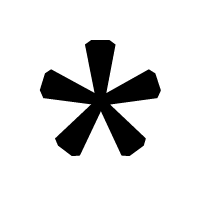
\includegraphics[width=0.25\textwidth]{../cases/ast/qb.pdf}}
  \caption{The shape progression of the template to the target, with the vectors
  field as defined on the curve}
  \label{fig:vectors}
\end{figure}
\fig{vectors} shows the progression of the deformation of a circle template
shape to an asterisk target shape. The optimiser required 44 function calls to
find the minimum $\vect u$, with $\int \vert \vect q(s,1) - \vect q_B(s)
\vert^2\,ds$ giving the residual as $0.0369$. The vector field is shown attached
directly on the shape, which show a greater magnitude towards the inner points
of the asterisk, as they are ``pulled in'' more quickly. The two shapes have a
similar parameterisation, as there is not a large amount of rotation along the
curve for the respective points to match.

\begin{figure}[!h]
  \centering
  \subfloat{\includegraphics[width=0.333\textwidth]{../cases/numbers/step_0.pdf}}
  %\subfloat{\includegraphics[width=0.333\textwidth]{../cases/numbers/step_1.pdf}}
  \subfloat{\includegraphics[width=0.333\textwidth]{../cases/numbers/step_2.pdf}}
  \subfloat{\includegraphics[width=0.333\textwidth]{../cases/numbers/step_3.pdf}}\\
  %\subfloat{\includegraphics[width=0.333\textwidth]{../cases/numbers/step_4.pdf}}
  \subfloat{\includegraphics[width=0.333\textwidth]{../cases/numbers/step_5.pdf}}
  \subfloat{\includegraphics[width=0.333\textwidth]{../cases/numbers/step_6.pdf}}
  %\subfloat{\includegraphics[width=0.333\textwidth]{../cases/numbers/step_7.pdf}}
  \subfloat{\includegraphics[width=0.333\textwidth]{../cases/numbers/step_8.pdf}} 
  \caption{Evolution of the a curve at selection of time steps showing the self
    intersection of the curve.}
\label{fig:intersection}
\end{figure}
An important feature of an approach based on inner metrics is shown in
\fig{intersection}, where the shape clearly intersects itself during its
evolution. This is possible since the deforming vector is directly applied to
the curve, leaving the ambient space unaffected. This is in contrast to LDDMM,
or other methods using outer metric which deform the entire space which cannot
self intersect.

\begin{figure}[!h]
  \centering
  \subfloat[$f(s)$ \label{fig:param_a}]{\includegraphics[width=0.25\textwidth]{../reparams/path_0.pdf}}
  \subfloat[$g(s)$ \label{fig:param_b}]{\includegraphics[width=0.25\textwidth]{../reparams/path_1.pdf}}
  \subfloat[$h(s)$ \label{fig:param_c}]{\includegraphics[width=0.25\textwidth]{../reparams/path_2.pdf}}
  \subfloat[$k(s)$ \label{fig:param_d}]{\includegraphics[width=0.25\textwidth]{../reparams/path_3.pdf}}\\
  \subfloat{\includegraphics[width=0.25\textwidth]{../reparams/steps_0.pdf}}
  \subfloat{\includegraphics[width=0.25\textwidth]{../reparams/steps_1.pdf}}
  \subfloat{\includegraphics[width=0.25\textwidth]{../reparams/steps_2.pdf}}
  \subfloat{\includegraphics[width=0.25\textwidth]{../reparams/steps_3.pdf}}\\
  \caption{Changes in path and shape evolution of four parameterisations of the
    same target shape. The top row shows the path taken by a selection of points,
    the bottom row shows the evolution of the template shape. Functions for the smaller circle (target) are shown in Tab. \ref{tab:funs}.}
  \label{fig:reparams}
\end{figure}
The parameterisation dependence of the penalty term is demonstrated in
\fig{reparams}, where the target shape is identical, but is parameterised
differently in each case. The problem is the scheme will move each particular
point on the template curve to its new location on the target curve, which is
not desired in computational anatomy.  If the penalty term was parameterisation
invariant, all of the paths and curve evolution in \fig{reparams} would be the
same, with equal distance travelled.

The shapes in \fig{reparams} were not created with the PNG tracing script, but
where defined with parametric equations. The template shape is $r(s) = (100\sin
s, 100\cos s)$ for each of the cases, with the respective functions of the
target shapes shown in Tab. \ref{tab:funs}. \fig{param_a} has the same
parameterisation as the target, but is scaled to half size. As expected, the
deformation involves simply shrinking the circle. The target is rotated by
$\frac{\pi}{4}$ in \fig{param_b}, the path taken by points on the curve account for this
rotation resulting in a long path than in \fig{param_a} despite the  evolution
of the deformation appearing similar to that in \fig{param_a}.

\begin{table}[!h]
\begin{tabular}[h]{l}
    $\quad\quad\quad\quad f(s) =  (50 \sin s,\quad 50 \cos s$) \\
    $\quad\quad\quad\quad g(s) =  (50 \sin (s + \frac{\pi}{4}),\quad 50\cos (s + \frac{\pi}{4})$)\\
    $\quad\quad\quad\quad h(s) =  (50 \sin 2s,\quad 50 \cos 2s$) \\
    $\quad\quad\quad\quad k(s) =  (50 \cos s,\quad 50 \sin s)$
 \end{tabular}
 \caption{Functions for the target shapes in \fig{reparams}, functions from top
   to bottom correspond with the shapes in \fig{reparams} from left to right.}
 \label{tab:funs}
\end{table}

The final two parameterisations result in more complicated paths and
deformations. Doubling the parameter $s$ as in \fig{param_c} results in the shape
collapsing on itself and twisting before expanding out into the target
shape. Swapping the functions for each dimension results in path and deformation
shown in \fig{param_d}, where the circle flattens out until collapsing through itself, before
expanding to the target, resulting in a target shape that is mirrored to that in
\fig{param_a}.

\begin{figure}[h!]
  \centering
  \subfloat{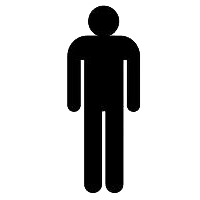
\includegraphics[width=0.333\textwidth]{../cases/people/qa.pdf}}
  \subfloat{\includegraphics[width=0.333\textwidth]{../cases/people/q_5.pdf}}
  \subfloat{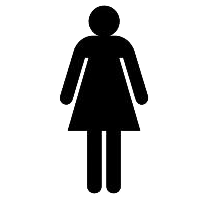
\includegraphics[width=0.333\textwidth]{../cases/people/qb.pdf}}
  %\subfloat{\includegraphics[width=0.333\textwidth]{../cases/people/quiver_0.pdf}}
  %\subfloat{\includegraphics[width=0.333\textwidth]{../cases/people/quiver_5.pdf}}
  %\subfloat{\includegraphics[width=0.333\textwidth]{../cases/people/quiver_9.pdf}}
  \caption{Shapes at $t=0$, $t=0.5$, and $t=1$, with the middle shape
    showing the average between}
\label{fig:average}
\end{figure}

Finding the geodesic between to shapes allows us to perform meaningful statistics from the
information gathered from deformation of images, in terms of both the value of
the functional $S[\vect u]$ and evolution of the shapes $\vect q(s,t)$. This
includes the ability to show an average between to shapes, as
demonstrated in \fig{average}. The initial shape $\vect q(s,0)$ is to the left,
with the final shape $\vect q(s,1)$ to the right. The middle shows the average
shape $\vect q(s,0.5)$, occurring half way through the time interval from $t=0$
to $t=1$. 

It is important to note that the average here is again dependent on
the parameterisation of the template and target curves. This is seen in the
asymmetry along the vertical axis of the average, which is not expected based on
symmetric nature of the template and target. If the penalty term was
parameterisation invariant, the average between these images should also be
vertically symmetric.


\subsection{Application demonstrations}

We can demonstrate both the viability and limitations of the Python code
by showing some simple test cases which are in similar in nature to how the
approach could be used for applications in computational anatomy.

\subsubsection{Shape identification\label{sec:shapematch}}

\begin{figure}[!h]
  \centering
  
\includegraphics[width=0.35\textwidth]{img/shapematch/test_star.png}
  \caption{The test shape: a hand drawn star which we attempt to identify as a known shape.}
  \label{fig:hand_star}
\end{figure}

For the first test, we attempt to identity a given curve from a small database
of known shapes. A crudely hand drawn shape (\fig{hand_star}), and the shape
database (\fig{shapedb}) are given as PNG files, which are individually send the
to tracing script, resulting in a set of plain text vector files. The test shape
is set as the template shape and is deformed into each of the shapes in the
database, storing the value of $S$ for each respective known shape.
\begin{figure}[!h]
  \centering
  \subfloat[]{
\includegraphics[width=.12\textwidth]{img/shapematch/circle.png}}\,
  \subfloat[]{
\includegraphics[width=.12\textwidth]{img/shapematch/hexagon.png}}
  \subfloat[\label{fig:pentagon}]{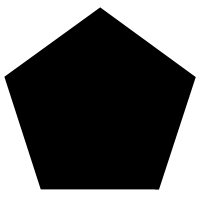
\includegraphics[width=.12\textwidth]{img/shapematch/pentagon.png}}
  \subfloat[]{
\includegraphics[width=.12\textwidth]{img/shapematch/square.png}}
  \subfloat[\label{fig:star}]{
\includegraphics[width=.12\textwidth]{img/shapematch/star.png}}
  \subfloat[]{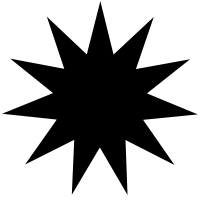
\includegraphics[width=.12\textwidth]{img/shapematch/star_11.png}}
  \subfloat[]{
\includegraphics[width=.12\textwidth]{img/shapematch/star_six.png}}
  \subfloat[]{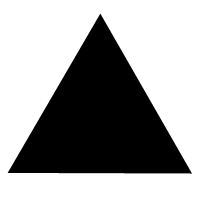
\includegraphics[width=.12\textwidth]{img/shapematch/triangle.png}}
  \caption{Set of known shapes which the test shape is matched against.}
  \label{fig:shapedb}
\end{figure}

The code was able to successfully identity the shape \fig{hand_star} as being
most similar to the star shape in \fig{star}. The deformation of the test shape
to each respective database shape is shown in \fig{shape_match}, along with the
value of the functional $S[\vect u]$. The values are normalised by the lowest
value of $S[\vect u]$, since the smallest value gives the shape which most closely
matches the given test shape,  when normalised, the identified shape has
$S[\vect u] = 1$. The second closest match, the pentagon (\fig{pentagon}), is
a reasonable suggestion, comparing both the value of $S$ and the deformation
progression in \fig{pentagon_deformation}.

Parameterisation of the curves does not greatly impact the ability of the code
to differentiate between types of shapes in this case because there large
differences between the shapes. Also, the algorithm used by
\texttt{bwboundaries()} to find the stating point for tracing the curve results
is roughly the same location for each of the shapes --- so the rotation to
account for the parameterisation is similar for each shape.

\begin{figure}[h!]
  \centering
  \subfloat[$S = 8.92$]{
\includegraphics[width=.333\textwidth]{img/shapematch/circle.pdf}}
  \subfloat[$S = 14.30$]{
\includegraphics[width=.333\textwidth]{img/shapematch/hexagon.pdf}}
  \subfloat[$S = 6.05$\label{fig:pentagon_deformation}]{\includegraphics[width=.333\textwidth]{img/shapematch/pentagon.pdf}}\\
  \subfloat[$S = 23.84$]{\includegraphics[width=.333\textwidth]{img/shapematch/square.pdf}}
  \subfloat[Match: $S = 1$]{\includegraphics[width=.333\textwidth]{img/shapematch/star.pdf}}
  \subfloat[$S = 8.93$]{\includegraphics[width=.333\textwidth]{img/shapematch/star_11.pdf}}\\
  \subfloat[$S = 12.31$]{\includegraphics[width=.333\textwidth]{img/shapematch/star_six.pdf}}
  \subfloat[$S = 16.48$]{\includegraphics[width=.333\textwidth]{img/shapematch/triangle.pdf}}
  \caption{Evolution of shape at each time step for each respective shape in the
    library. Normalised with the lowest value of $S$, matching shape is where $S
  = 1$.}
  \label{fig:shape_match}
\end{figure}

A limitation with the current code is that scale and translation is not
accounted for, as it assumed the test image shares a similar size and position
with those in the database. If the test image is significantly larger or
positioned away from the known images, the quality of the result would be
questionable. This could be improved by applying a translation to the test image
if needed before running the existing matching code.

%\clearpage
\subsubsection{Typeface classification \label{sec:fonts}}
A more difficult test application was devised to see how well the matching
scheme performed with less variation between shapes. In this test, we are
interested the classification of typefaces between \emph{serif} and
\emph{sans-serif}. Serifs are small structures on the ends of certain letter
strokes to improve the readability of printed text. 

\begin{figure}[h!]
  \centering
  \includegraphics[width=0.6\textwidth]{img/serifs.pdf}
  \caption{The left side shows a serif typeface with serifs circled in red. A
    sans-serif typeface is on the right.}
\label{fig:serif-demo}
\end{figure}

Typefaces with letters containing serifs are categorised as serif typefaces, and
those without are considered sans-serif typefaces. \fig{serif-demo} shows a
serif typeface on the left, with the serifs circled in red, the lack of such
features is noticeable in the sans-serif typeface on the right. A typeface with
characters set at a specific size is known as a \emph{font}.

For the test, an image of the uppercase letter ``N'' from a library of $22$
equally sized typefaces, $11$ serif and $11$ sans-serif fonts, was created. The
images were then converted to parameterised curves using the PNG tracing tool.


Each font is matched against the other 21 fonts in the library, and the
average values of $S[\vect u]$ found for deformations of the current test font
to those in the serif and sans-serif categories. The category with the lowest
average deformation indicates the class of the test font.

All eleven sans-serif fonts were successfully classified, as each sans-serif font
required a smaller deformation relative to each other. In \fig{font_right}, the
Helvetica font is deformed into the sans-serif Arial and serif Times New Roman
fonts. From visual inspection it can seen Helvetica is more similar to Arial
than Times New Roman, which is the case for the other fonts as the average $S$
when deforming Helvetica into the other sans-serif fonts is less than the
average deformations to serif fonts, suggesting that Helvetica is indeed a
sans-serif font.

\begin{figure}[h!]
  \centering
  \subfloat[Helvetica $\rightarrow$ Arial]{\includegraphics[width=0.5\textwidth]{img/helvetica/sans-arial.pdf}}
  \subfloat[Helvetica  $\rightarrow$ Times New Roman]{\includegraphics[width=0.5\textwidth]{img/helvetica/serif-times.pdf}}
  \caption{Helvetica is successfully classified as a \emph{sans-serif} font.}
  \label{fig:font_right}
\end{figure}

While initial results were promising when classifying sans-serif fonts, only $5$
of $11$ the serif fonts successfully were classified as such. \fig{sabon}
suggestions this is likely again due to the parameterisation dependence of the
penalty term in \eq{S}. Here, it appears that Times New Roman and Sabon are more
similar than Time New Roman is to Arial. 

\begin{figure}[h!]
  \centering
  \subfloat[Times New Roman  $\rightarrow$ Arial]{\includegraphics[width=0.5\textwidth]{img/times/sans-arial.pdf}}
  \subfloat[Times New Roman  $\rightarrow$ Sabon\label{fig:sabon}]{\includegraphics[width=0.5\textwidth]{img/times/serif-sabon.pdf}}
\caption{Times New Roman is inaccurately classified as a \emph{sans-serif} font.}
  \label{fig:font_wrong}
\end{figure}

The progression of the deformation in \fig{sabon} shows the curve rotating,
contacting, and expanding, resulting in a large deformation that skews the
average deformation among similar classed fonts. Several of the serif fonts
where parameterised significantly differently by the PNG tool, hence the results
of the test unreliable at best, and at worst completely invalid. It is likely
increasing the font library more carefully parameterising the letters would
give more accurate typeface classifications.
 

\section{Conclusions\label{sec:conc}}

A numerical scheme to find an approximate geodesic between two shapes is
presented. Unlike outer metric methods, which deform the space itself, we use
inner metrics to attach a deforming vector to the shape directly. A functional
$S[\vect u]$, composed of a metric and penalty term, is defined such that when
minimised using a BFGS optimisation algorithm a geodesic (to computational
accuracy) is found. A gradient for the functional $S[\vect u]$ is derived
and is used to aid in the convergence of the optimisation algorithm.

The scheme is implemented as a Python code, making heavy use of libraries from the FEniCS project,
which facilitate the finite element solutions used in the code.

The current code is best suited for cases where the specific parameterisation of the
template and target are important. Unfortunately, most curves in computational
anatomy are unparameterised, and the interest is only in finding the geodesic
between generalised shapes, not curves with a specific parameterisation.

The code works well for cases where registered images are matched against shapes
with large variation, such as the shape identification experiment in Sec.
\ref{sec:shapematch} When used in applications similar to Sec. \ref{sec:fonts}
that are more sensitive to the curve parameterisations the geodesics found are
of dubious use. Most parameterisation issues seen in Sec. \ref{sec:experiments} are due to the automatic
parameterisation in the PNG tracing tool, these problems would likely be reduced
if the curves  were  parameterised  more carefully. 

However, it would be more desirable if the geodesic found by code was
parameterisation invariant, as it is likely the non-trivial shapes encountered
in ``real world'' applications would be sourced from medical imaging equipment
and difficult to manually reparameterise to eliminate the extra error in the
penalty term caused by the parameterisation dependence. This step of manual
intervention also interferes with what should be a completely automated process.


We could improve the functional $S$ by replacing the penalty term with one that
is completely parameterisation invariant, assuming one could be found that did
not involve a reparameterisation of either curve. Alternatively, the penalty
term could be replaced with a matching condition that incrementally applies a
reparameterisation during the evolution of the curve as in
\cite{cotter2009geodesic}. Another possibility is to apply an explicit
reparameterisation velocity to initial curve as introduced in
\cite{clark2011reparam}, this approach still allows a particular
parameterisation of the target to be specified.


In the currently implementation, the translation of the shape is included in the
penalty term. For example, if this was not the case, an the template and target
were identical circle, but with different centres, zero deformation could be
required. Large translations could be ignored by finding the centroid of each
shape and moving a curve such that location of both centroids is shared when the
solver is initialised. If computing the centroids is difficult, or
computationally expensive, pre-alignment of the curves could be achieved by
using a bounding box around each respective shape, and then translating an image
so that the centre of both bounding boxes are equal. Alternatively, we could
modify terms to the functional \eq{S} to account for translation without
incurring penalty, which would not require and modifications of the curves when
initialising the problem.

The code could improved by adding a method to find the value of
$\sigma$ which would reduce the trial and error approach of prescribing a
$\sigma$ and changing it and needed to improve the results. By staring with a
reasonably large $\sigma$ and performing the deformation, the code could
successively reduce $\sigma$ until an acceptable residual between $\vect q(s,1)$ and
$\vect q_B(s)$ is reached. Important to this approach is that the velocity found at each these iterations can be used as
the initial guess of $\vect u(s,t)$  when starting the
optimiser with a new value of $\sigma$, which would reduce the performance
impact of automating the selection of $\sigma$.

Because of the storage requirements involved in each iteration of the optimiser,
the current approach of finding the geodesic may not be optimal for larger
problems requiring a more refined mesh or greater time steps. The use of inner
metrics could be adapted to define a problem where we find the initial
conditions to give the geodesic from a curve momentum equation. This would be
similar to the geodesic shooting method commonly used with outer metrics
\cite{miller2006geodesic, cotter2009geodesic, clark2011reparam}.


The results show that the inner metric approach is valid and warrants further
investigation, particularly regarding possible improvements of the penalty
term. The code works within the known limitations of the scheme and should serves as
a good starting point for continued development.


\newpage
\addcontentsline{toc}{section}{References}
\bibliographystyle{unsrt}
\bibliography{refs}{}
\end{document}